\documentclass[11pt,a4paper]{article}
\usepackage[margin=22mm]{geometry}
\usepackage{tikz}
\usetikzlibrary{positioning,arrows.meta}
\usepackage[hidelinks]{hyperref}
\title{Course module compilation: aliases, Unicode, paths and source provenance}
\date{Created-at: 2026-09-09 13:36 +02:00}
\begin{document}
\maketitle
\paragraph{Scope and ETA.} Implement the four downstream findings in priority order,
through the real Node/browser WASM SDK. Estimate after Core approval: 2--3 hours,
approximately 50 minutes module composition, 30 minutes source metadata and wire
compatibility, 20 minutes lexer/path controls, 40--80 minutes owner and SDK builds.
This is not a performance campaign. Exact downstream material is not available;
use the report's minimal reproductions and discriminating controls.
\paragraph{Evidence.} Current packaged WASM succeeds with course as entry and with
an index that imports concepts first; lecture importing course fails on
\texttt{prod.production\_concept}. Nested parent imports fail on the uncollapsed
virtual path. Escaped UTF-8 is corrupted; plain strings work. Inspect contains no
declaration-to-file mapping. Local dirty parser already contains the byte-preserving
escape fix, which has not reached the SDK. Reuse that fix and strengthen its tests.
\paragraph{Owners and reviewable implementation.} Core ModuleStore must enumerate
the complete reachable import graph deterministically, retaining existing direct
import order and deduplicating shared module instances. Resolve each module's
using statements against its own imports; preserve module-local alias environments
instead of merging into a process-wide map or ignoring resolution errors. The
resolution owner must prevent aliases leaking between unrelated modules, including
two modules using the same alias for different dependencies. Preserve the existing
public lowering entry points; share the implementation where a context is needed.
Core SourceProvider normalizes joined paths before cache and file lookup, collapses
dot segments and rejects traversal above a virtual root. Filesystem canonicalization
continues to resolve real paths, including valid parent imports and symlinks; no new
project-directory sandbox is implied. Parser common lexer retains its borrowed
escape-free fast path and byte-preserving owned escape path.
\paragraph{IR and SDK contract.} Add optional serialized \texttt{files: string[]}
and \texttt{decl\_file: u32[]} to IR. For compiler-produced IR every declaration,
including anonymous arcs, maps to a valid source-file table entry. Legacy payloads
without either field remain readable. Validate lengths and file indices together;
reject inconsistent metadata. Preserve provenance in JSON/CBOR round trips and
declaration-allocation paths; explicitly represent unknown provenance for synthetic
declarations rather than inventing a source. Source metadata is excluded from
structural and semantic hashes. SDK inspect exposes these additional IR keys;
compile/compileFiles/inspect signatures and schemaVersion remain unchanged.
\paragraph{Hash compatibility.} Freeze successful single-file and direct-import
structural hashes before the fix. Metadata must not alter them. Corrected transitive
compilation can include previously omitted declarations and thus change topology
and hash; report this explicitly. Structural hash is not a content digest: two
documents differing only in string values already have the same structural hash.
Serialized IR bytes gain metadata; do not claim unchanged bytes or silently replace
the existing frozen-byte tests. Retain a legacy-field projection control plus new
provenance round-trip assertions.
\paragraph{Affected files.} Core: this four-file plan; docs/ir-source-provenance.md;
module\_store/module\_store.rs,
module\_store/source\_provider.rs, resolution/resolve.rs, ir/lower.rs, ir/ir.rs,
ir/coherence.rs and writers/cbor\_writer.rs under hymeko\_core/src as required for
the existing wire validators; existing module-store tests, unified\_ir verification
and CBOR tests under hymeko\_core/tests; Cargo.toml/Cargo.lock parser pin; generated
SYMBOLS.md; IR consumer documentation and task report. Parser: src/lexer/common.rs
only the existing Unicode bugfix for release; tests/simd\_lexer\_tests/simd\_lexer\_tests.rs;
task report. Web: Cargo.toml/Cargo.lock exact provider pins; existing
crates/hymeko\_wasm/src/document.rs tests if needed; tests/sdk.test.mjs and existing
native/browser parity harness; packages/hymeko/src public inspection types if
needed; README/changelog; generated SDK dist/wasm/packed archive and task report.
Additional checked test boundary: hymeko\_core/tests/unified\_ir/validation/cbor\_roundtrip.rs
expects 103 successful documents, while the original 102-document hash KAT remains
intact. Web native parity example adds a test-only compile-files stdin mode.
\paragraph{Inherited gate drift.} The published Core base f305ade already has a
stale SYMBOLS.md (670 recorded versus 713 extracted symbols) and duplication
baseline (429 clones / 8332 lines versus 460 / 9481 measured on the untouched base).
Before formatting the fixes measure 460 / 9480; after scoped rustfmt they measure
460 / 9481, identical to the published base: no new clones or cloned lines.
Refresh generated SYMBOLS.md and .duplication-baseline.json only after this
controlled base comparison; no WGPU source is changed. This is a documented
reconciliation of the published base, not an exemption for new duplication.
\paragraph{Core protection.} Scope identifier presented in the approval request:
\texttt{APPROVED-CORE-EDIT: course-module-compilation}. The user explicitly approved
that request in chat: ``persze ez most nagyobb feladat mehet''. This is approval of
the exact named scope, not a claim that the user typed the literal token. The
user's explicit authorization takes precedence over repeating the local ceremony.
Protected items are Core
library sources and its parser dependency pin. Existing compiler-repeated-work
approval did not cover changed import semantics or new IR metadata. Before this
approval only allowlisted tests, documentation, read-only investigation and Parser
regressions were changed. Do not change CORE.YAML to grant ourselves approval.
\paragraph{Git isolation.} Fresh fetch succeeded in Core, Parser and Web on this
task. Core published SDK base and github/main are f305ade; origin/main advanced
to 262fc0b with unrelated sparse/WGPU changes. Parser published base is 284c490;
Web github/main is 8d4050a. Preserve staged report removals, unpublished parser/Core
performance work and Web theme/graph changes. No reset, stash or broad staging.
For the isolated bugfix release, two simultaneous independent branches are needed:
unfinished performance work stays in the existing checkouts while only course fixes
are published on fix/course-module-compilation. Reusing the Python integration
worktree would disturb a third independent branch. Create sibling checkouts
core-course-release (base f305ade) and parser-course-release (base 284c490), owned
by this task; remove after verified SDK delivery only if clean and fully published,
otherwise report their state. They share the existing ../hymeko contract provider.
The Core release is intentionally isolated from the Gitea sparse development line.
Refresh and compare again before publication. No public site
deployment is included. Deliver the packed SDK and verified exact provider pins;
update a downstream vendor copy only after locating its actual checkout/contract.
\paragraph{Tests.} Core: real parser, course/lecture/index entry permutations,
transitive and diamond imports, aliases with equal names in different modules,
invalid using diagnostics, normalized equivalent paths, above-root failures,
cycles, metadata completeness and legacy/malformed JSON/CBOR. Controls: edge as
edge member; DeclId differs from NodeId in multi-file input; frozen structural
hashes. Parser: escaped Hungarian/Japanese before and after escapes, escaped
non-ASCII, all supported escapes, combining marks/emoji, borrowed no-escape path,
byte spans and unterminated errors, scalar and supported SIMD variants. First run
regressions against old behavior; failures must match the reported defect. Then
full relevant owner suites and portable symbols/duplication/preflight gates,
scoped rustfmt/clippy. Web: native/WASM parity, npm run build, npm test,
npm run pack:sdk; inspect the packed tarball through a fresh SDK import. Pin
wasm-bindgen CLI 0.2.127. Do not claim a downstream site rebuild without executing it.
\paragraph{Budgets and risks.} Keep SDK 64-file, 1 MiB input and 10,000-declaration
limits, including transitive imports. Avoid cloning the full index per module or
exponential diamond expansion. Module graph work linear in reachable input plus
bindings; provenance approximately 4 bytes per declaration plus distinct file names.
Process peak working set below 16 GiB; stop a build exceeding that budget. Cyclic
imports, repeated aliases, many tiny files and near-cap declaration counts are the
adversarial cases. Cache keys must use canonical provider paths. No performance
claim without an affected-path measurement. Report unmeasured limits honestly.
\paragraph{Rollback and acceptance.} Revert only the dedicated bugfix commits and
restore exact consumer pins/archive; preserve pre-existing dirty work. Completion
requires owner regressions passing, packed WASM tests passing, compatibility notes
and delivered SDK artifact. Record test failures and approval/build blockers without
claiming implementation success. Write reports and verify incremental Samba archival
using the provider report\_sync tool before closing the task.
\begin{center}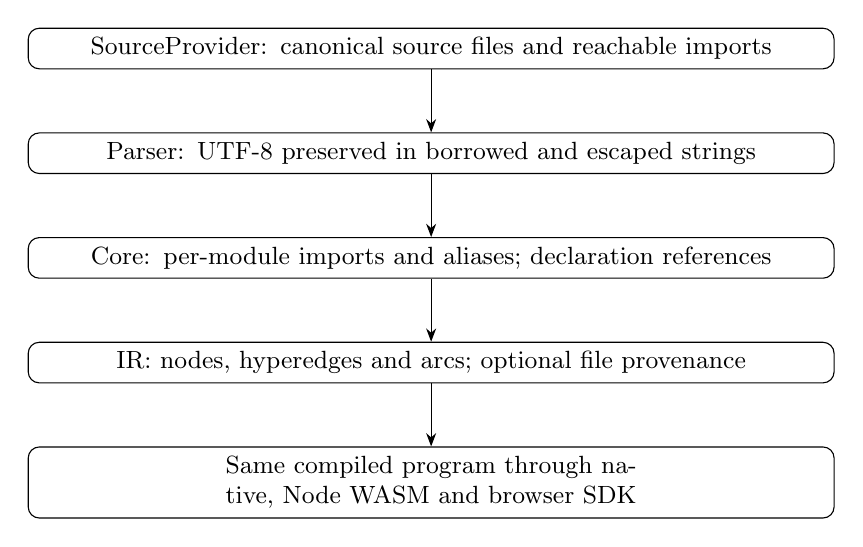
\begin{tikzpicture}[node distance=8mm, every node/.style={draw,rounded corners,align=center,font=\small,text width=10cm}, >=Stealth]
\node (source) {SourceProvider: canonical source files and reachable imports};
\node[below=of source] (parse) {Parser: UTF-8 preserved in borrowed and escaped strings};
\node[below=of parse] (resolve) {Core: per-module imports and aliases; declaration references};
\node[below=of resolve] (ir) {IR: nodes, hyperedges and arcs; optional file provenance};
\node[below=of ir] (sdk) {Same compiled program through native, Node WASM and browser SDK};
\draw[->] (source)--(parse); \draw[->] (parse)--(resolve);
\draw[->] (resolve)--(ir); \draw[->] (ir)--(sdk);
\end{tikzpicture}
\end{center}
\end{document}
